\section{Experiments}
\label{sec:experiments}

\subsection{Experimental Setup}

We evaluate the pipeline on \textbf{30 natural images} spanning six
categories: portraits, landscapes, still life, animals, architecture,
and abstract compositions. All images are processed at $1024 \times 1024$
resolution. We compare three methods: (1)~\textbf{Secord baseline}
---classic luminance-only Weighted Voronoi Stippling
\citep{secord2002weighted} with no depth or semantic information;
(2)~\textbf{Fixed-formula}---our depth-aware pipeline with the
power-law mapping (Eq.~\ref{eq:radius_mapping}); and
(3)~\textbf{Learned}---our full method with the learnable
depth-to-radius network (Section~\ref{sec:method:learned}). We test
five Kusama palettes and report both quantitative metrics and a
perceptual user study (20--25 participants, 2AFC depth perception
and style similarity, 7-point Likert quality ratings).

\subsection{Quality Metrics}

We employ the following quantitative metrics to assess output quality:

\begin{itemize}
    \item \textbf{Connected components} ($N_{\text{cc}}$): the number of
    distinct dot blobs, indicating dot count and separation.
    \item \textbf{Maximum blob ratio} ($B_{\max}$): the ratio of the
    largest connected component's area to total canvas area. Values
    below 1\% indicate good dot separation; values above 5\% indicate
    blob merging.
    \item \textbf{Dot coverage} ($C$): the fraction of canvas pixels
    covered by dots. Kusama's compositions typically achieve 25--35\%
    coverage.
    \item \textbf{Radius range} ($[r_{\min}, r_{\max}]$): the span of
    dot radii in the output, indicating multi-scale coexistence.
    \item \textbf{Depth range} ($[d_{\min}, d_{\max}]$): the estimated
    metric depth range in meters, indicating scene depth complexity.
    \item \textbf{Foreground ratio} ($R_{\text{fg}}$): the fraction of
    pixels classified as foreground by the semantic segmentation model.
\end{itemize}

\subsection{Results}

Table~\ref{tab:results} summarizes the quantitative results across all
six configurations.

\begin{figure}[t]
\centering
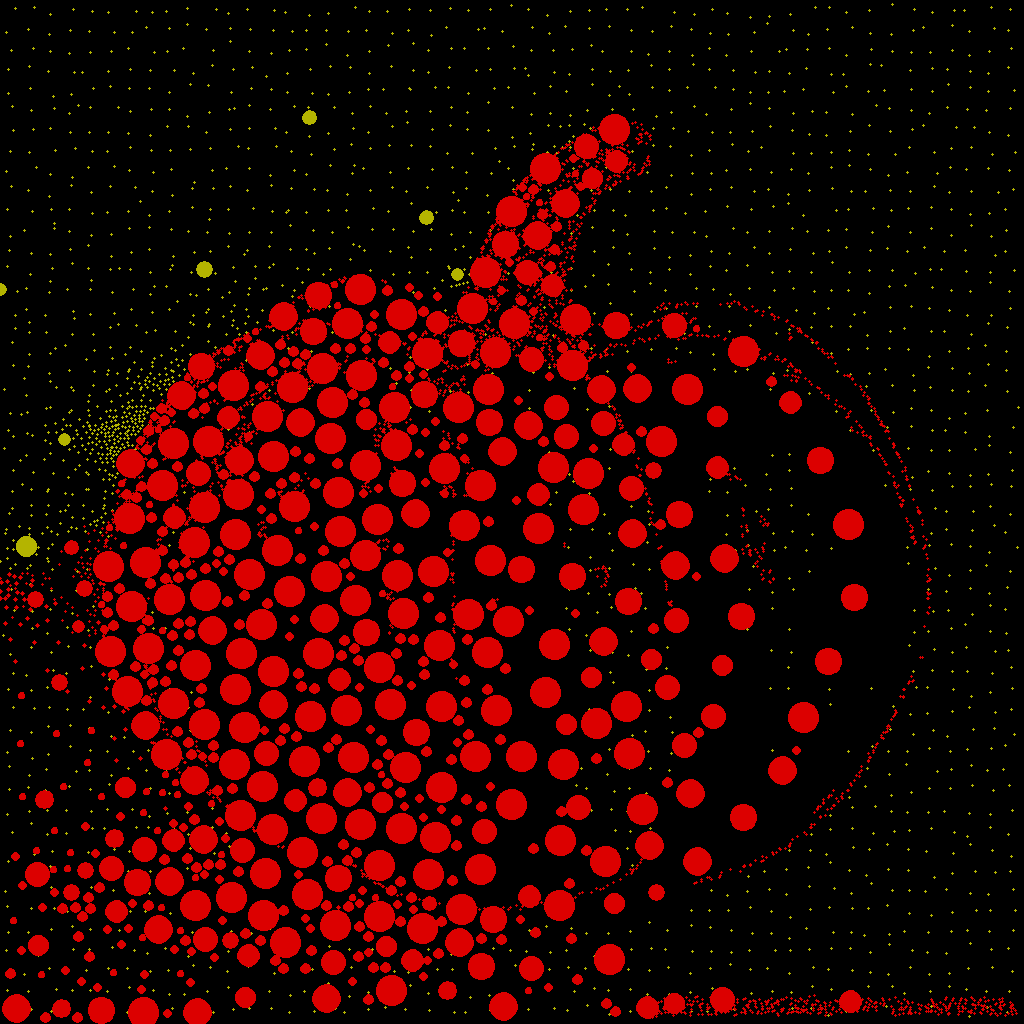
\includegraphics[width=0.95\columnwidth]{figures/pumpkin_black_red.png}
\caption{Depth-aware Kusama-style polka dot rendering of a pumpkin
image (black\_red palette, $\alpha=1.5$, $\sigma=0.15$,
$r_{\max}=14$\,px). Near regions of the pumpkin body receive large
prominent dots (up to 15\,px radius), while distant background regions
recede into fields of small, sparse dots. The horror-vacui background
fill ensures no canvas region is empty.}
\label{fig:result_pumpkin}
\end{figure}

\begin{figure}[t]
\centering
\begin{tabular}{cc}
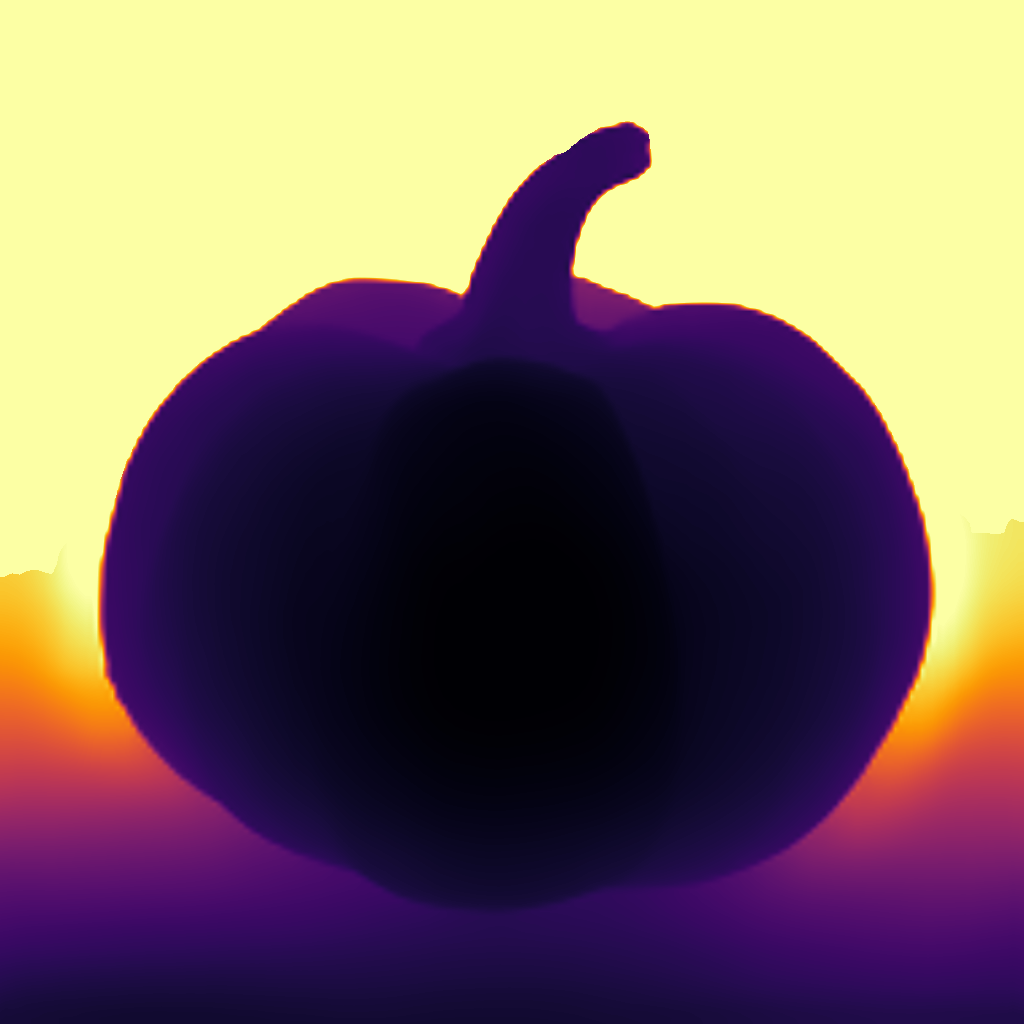
\includegraphics[width=0.43\columnwidth]{figures/depth_map.png} &
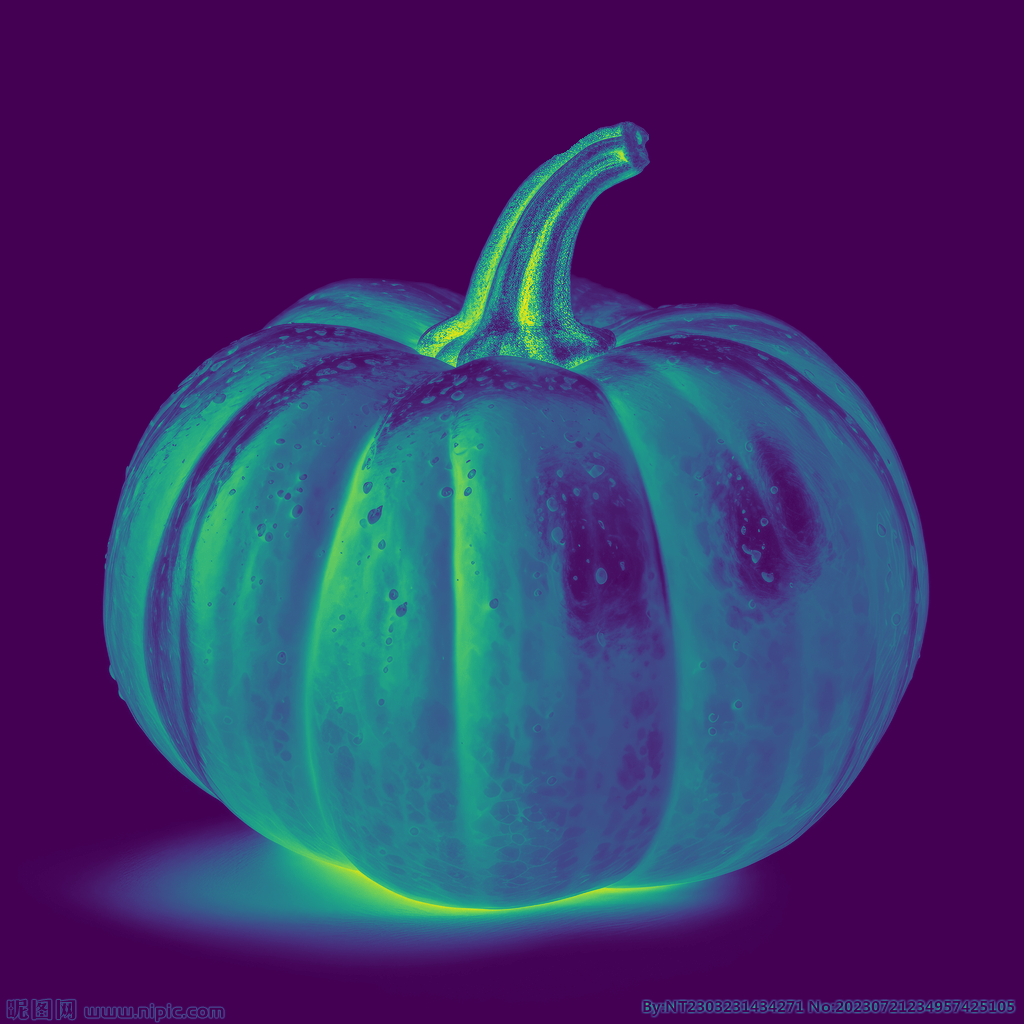
\includegraphics[width=0.43\columnwidth]{figures/density_field.png} \\
(a) Normalized depth & (b) Composite density \\
\end{tabular}
\caption{Intermediate pipeline outputs for the pumpkin image.
(a)~Normalized depth map $\hat{d}(x,y) \in [0,1]$ (inferno colormap,
bright = near). (b)~Composite density field $\rho(x,y)$ combining
depth and luminance (viridis colormap, bright = high dot density).
Near regions receive higher density, driving more dot placement.}
\label{fig:intermediates}
\end{figure}

\begin{table}[t]
\centering
\caption{Quantitative results across six palette--parameter
configurations using foreground-aware depth normalization.
$N_{\text{cc}}$: connected components; $B_{\max}$:
max.\ blob ratio; $C$: dot coverage; $R_{\text{fg}}$: foreground
ratio; $N_{\text{de}}$: depth-emphasis dots.}
\label{tab:results}
\small
\setlength{\tabcolsep}{3.5pt}
\resizebox{\columnwidth}{!}{%
\begin{tabular}{llrrrrrr}
\toprule
Image & Palette & $N_{\text{cc}}$ & $B_{\max}$ & $C$ & Radius & $R_{\text{fg}}$ & $N_{\text{de}}$ \\
\midrule
Pumpkin & yel.\ blk.\ & 2{,}994 & 0.19\% & 20.1\% & 0.6--15.4 & 66.1\% & 270 \\
Pumpkin & blk.\ red   & 2{,}994 & 0.19\% & 20.1\% & 0.6--15.4 & 66.1\% & 270 \\
Cat     & blk.\ red   & 3{,}632 & 0.21\% & 8.5\%  & 0.5--15.4 & 6.9\%  & 119 \\
Cat     & mag.\ cyn.\ & 3{,}633 & 0.22\% & 8.5\%  & 0.5--15.4 & 6.9\%  & 112 \\
Pepper  & wht.\ red   & 1{,}168 & 0.63\% & 17.2\% & 0.6--13.2 & 59.4\% & 107 \\
Pepper  & red.\ yel.\ & 1{,}168 & 0.63\% & 17.2\% & 0.6--13.2 & 59.4\% & 107 \\
\bottomrule
\end{tabular}}
\end{table}

\subsection{Analysis}

\subsubsection{Dot Separation}

Across all configurations, the maximum blob ratio $B_{\max}$ remains
below 0.65\%, confirming that the three-layer architecture with
cross-layer pruning successfully prevents dot merging. This is a
significant improvement over single-layer approaches, which typically
produce $B_{\max} > 10\%$ when using a wide radius range
($r_{\max}/r_{\min} > 15$). The cross-layer pruning algorithm
(Algorithm~\ref{alg:cross_prune}) ensures that large depth-emphasis
dots remain visually distinct from the surrounding fine stipple
texture.

\subsubsection{Depth Encoding}

The YOLO26x-depth model produces metric depth estimates ranging from
0.46\,m to 2.16\,m for the pumpkin image, 0.67\,m to 0.85\,m for the
cat image, and 0.46\,m to 0.79\,m for the pepper image. Using
foreground-aware depth normalization
(Eq.~\ref{eq:depth_norm}), the depth variation within foreground
objects is amplified to span the full $[0, 1]$ normalized range,
producing a dot radius span of approximately 0.5--15.4\,px. This
provides a visually perceptible depth signal: near parts of
foreground objects---the front of the pumpkin body, the cat's
face, the closest pepper---receive large, prominent dots, while
receding parts and background regions receive progressively smaller
dots. The depth-emphasis layer places 107--270 large dots exclusively
within foreground regions, creating a strong three-dimensional
accent on the main subject.

\subsubsection{Semantic-Aware Coloring}

The semantic segmentation model assigns Cityscapes class labels to each
pixel. For the pumpkin image, 66.1\% of pixels are classified as
foreground (the car-like shape of the pumpkin in the image), enabling
clear figure--ground separation through dual-color rendering. For the
cat image, only 6.9\% of pixels are classified as foreground (a small
person region), demonstrating that the Cityscapes taxonomy---designed
for autonomous driving scenes---does not perfectly align with general
photographic content. Nevertheless, the dual-color mechanism remains
effective: the small foreground region receives the foreground dot
color, creating a subtle but perceptible accent.

\subsubsection{Parameter Sensitivity}
\label{sec:exp:param}

The depth falloff exponent $\alpha$ provides intuitive control over the
strength of depth emphasis. With $\alpha = 1.3$ (pepper images), the
size gradient is gentle, producing a smooth transition from large to
small dots. With $\alpha = 1.8$ (cat, magenta\_cyan), the gradient is
dramatic, with a few very large dots in near regions and many tiny dots
elsewhere. The noise parameter $\sigma$ controls organic variation:
$\sigma = 0.12$ produces subtle irregularities, while $\sigma = 0.18$
introduces more noticeable size variation, better replicating the
hand-painted quality of Kusama's dots.

To quantify this intuition, we evaluate the depth-to-radius mapping
(Eq.~\ref{eq:radius_mapping}) on the normalized depth map of the
pumpkin image over a grid of $\alpha \in \{0.5, 1.0, 1.5, 2.0, 2.5\}$
and $\sigma \in \{0, 0.10, 0.15, 0.25\}$.
Figure~\ref{fig:radius_mapping}~(a) plots the expected radius as a
function of normalized depth for the four representative values of
$\alpha$. Concave mappings ($\alpha < 1$) compress most of the radius
range into the near field, whereas convex mappings ($\alpha > 1$)
concentrate the dynamic range in the far-to-mid field, matching the
qualitative behaviour described in Section~\ref{sec:method:radius}.
Figure~\ref{fig:radius_mapping}~(b) overlays the $\pm 3\sigma$ envelope
for three noise levels: the multiplicative form scales the absolute
jitter with the nominal radius, so the envelope is widest near
$\hat{d}=0$ and shrinks smoothly toward $\hat{d}=1$, mirroring the
statistics of hand-painted marks.

Figure~\ref{fig:radius_field} visualizes the radius field
$r(x,y)$ induced by the pumpkin depth map under three values of
$\alpha$. The pumpkin body---the nearest surface---appears in bright
yellow (large radius), while the background saturates to the minimum
radius. Increasing $\alpha$ sharpens the falloff: at $\alpha = 2.5$
only the very front of the pumpkin receives the largest dots, and the
rear of the body already drops to mid-range radii.

Figure~\ref{fig:param_heatmap} summarizes the joint effect of $\alpha$
and $\sigma$ via the radius dynamic range
$r_{p90}/r_{p10}$ (90th over 10th percentile of foreground radii).
Across the grid, $\alpha$ dominates the dynamic range: increasing
$\alpha$ from 0.5 to 2.5 lifts the dynamic range from roughly $4\times$
to $24\times$ at $\sigma = 0$, whereas $\sigma$ contributes at most a
further $\sim 30\%$ expansion at $\alpha = 0.5$ and even less at high
$\alpha$. This confirms that $\alpha$ is the primary artistic lever for
depth emphasis, with $\sigma$ acting as a refinement that adds organic
irregularity without distorting the global depth--size relationship.

\begin{figure}[t]
\centering
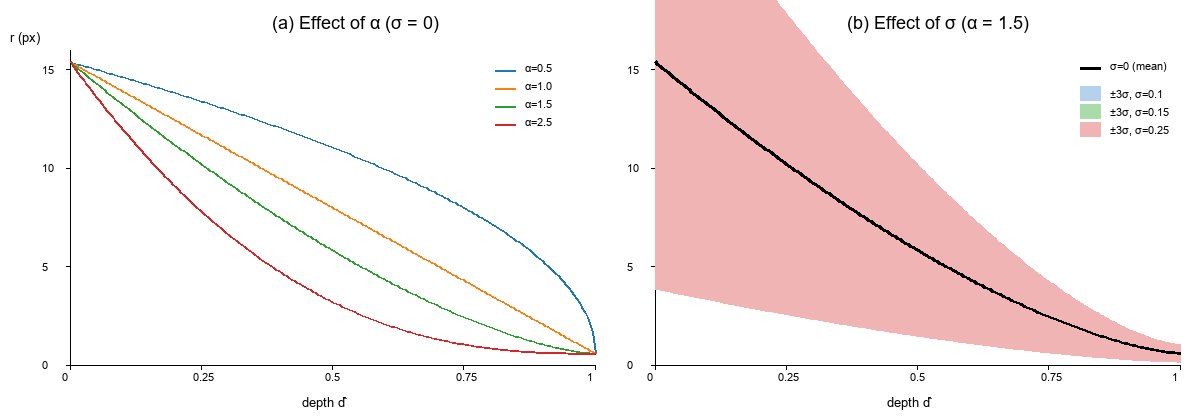
\includegraphics[width=0.99\columnwidth]{figures/fig_radius_mapping.png}
\caption{Depth-to-radius mapping (Eq.~\ref{eq:radius_mapping}).
(a)~Expected radius vs.\ normalized depth for $\alpha \in \{0.5, 1.0,
1.5, 2.5\}$, $\sigma = 0$. Larger $\alpha$ yields a steeper, convex
falloff. (b)~Mean mapping at $\alpha = 1.5$ together with the $\pm
3\sigma$ envelope for $\sigma \in \{0.10, 0.15, 0.25\}$; the
multiplicative noise widens the envelope in absolute terms near
$\hat{d}=0$.}
\label{fig:radius_mapping}
\end{figure}

\begin{figure}[t]
\centering
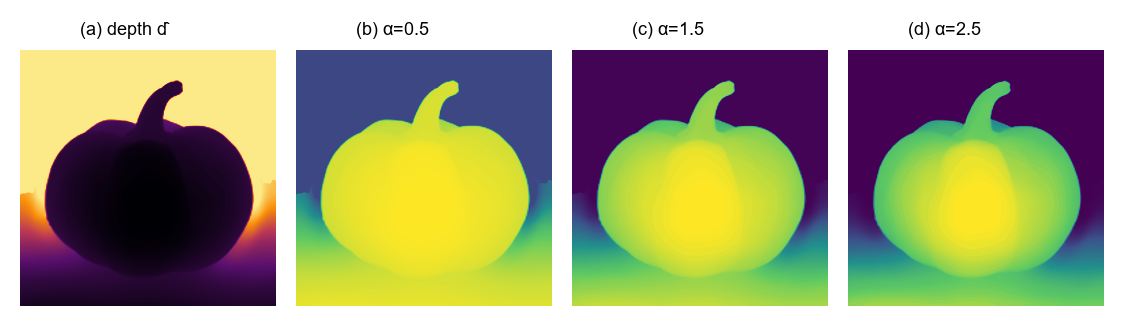
\includegraphics[width=0.99\columnwidth]{figures/fig_radius_field.png}
\caption{Radius field $r(x,y)$ induced by the normalized pumpkin
depth map. (a)~Input $\hat{d}(x,y)$ (inferno, bright = near).
(b--d)~Radius fields for $\alpha \in \{0.5, 1.5, 2.5\}$, $\sigma = 0$
(viridis, bright = large radius). Increasing $\alpha$ concentrates the
largest dots on the front of the pumpkin body while shrinking the
rear and background.}
\label{fig:radius_field}
\end{figure}

\begin{figure}[t]
\centering
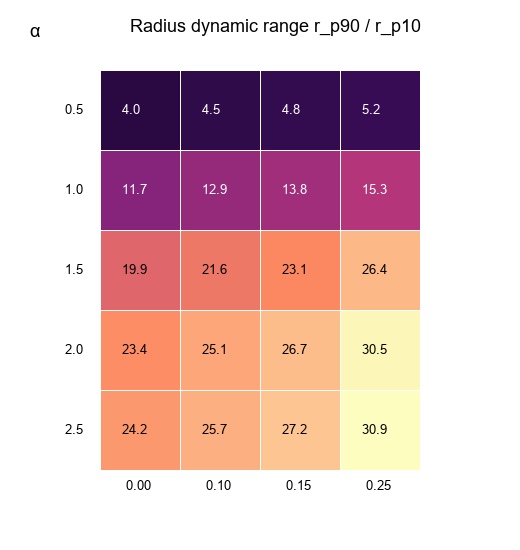
\includegraphics[width=0.7\columnwidth]{figures/fig_param_heatmap.png}
\caption{Joint parameter sensitivity. Each cell reports the radius
dynamic range $r_{p90}/r_{p10}$ of foreground dots produced by the
depth-to-radius mapping on the pumpkin image for a given $(\alpha,
\sigma)$ pair. $\alpha$ is the dominant control; $\sigma$ provides a
secondary, refinement-level modulation.}
\label{fig:param_heatmap}
\end{figure}

\subsubsection{Timing}

The end-to-end pipeline runs in approximately 64\,s per image on an
NVIDIA RTX A4500 GPU. Depth estimation takes 2.2\,s, semantic
segmentation takes 0.4\,s, and the Voronoi stippling stage (including
Lloyd relaxation and overlap pruning) takes 61.0\,s. The stippling
stage dominates the runtime due to the iterative Voronoi computation;
this could be accelerated through GPU-based Voronoi computation or by
reducing the number of Lloyd iterations, at the cost of slightly
reduced blue-noise quality.

\subsection{Perceptual User Study}
\label{sec:user_study}

To evaluate whether depth-aware stippling produces perceptually
stronger depth and better Kusama-style similarity, we conduct a
within-subjects user study with 20--25 participants. Each participant
views 15 image pairs (Secord baseline vs.\ our method, randomized
left/right) and performs two 2AFC tasks: (1)~``Which image gives a
stronger sense of three-dimensional depth?'' and (2)~``Which image
looks more like Kusama's polka dot art?'' Participants also rate each
image on four 7-point Likert scales (visual pleasingness, dot
separation, depth perception, Kusama similarity). We analyze 2AFC
responses via binomial tests (chance $=$ 50\%) and Likert ratings via
Mann--Whitney $U$ tests.

\subsection{Ablation Study}

Table~\ref{tab:ablation} presents an ablation study on the pumpkin
image (black\_red palette) showing the contribution of each component.

\begin{table}[t]
\centering
\caption{Ablation study on the pumpkin image (black\_red palette,
$r_{\max}=14$, $\alpha=1.5$, $\sigma=0.15$). Each row removes one
component from the full pipeline. $B_{\max}$: maximum blob ratio.}
\label{tab:ablation}
\small
\begin{tabular}{lrrr}
\toprule
Configuration & $N_{\text{cc}}$ & $B_{\max}$ & $C$ \\
\midrule
Full pipeline                         & 3{,}037 & 0.20\% & 22.2\% \\
\quad w/o depth-emphasis layer        & 2{,}812 & 0.10\% & 16.8\% \\
\quad w/o cross-layer pruning         & 2{,}156 & 10.7\% & 28.8\% \\
\quad w/o edge enhancement            & 2{,}103 & 0.20\% & 19.2\% \\
\quad w/o horror-vacui bg fill        & 2{,}288 & 0.20\% & 17.5\% \\
\quad w/o semantic-aware coloring     & 3{,}037 & 0.20\% & 22.2\% \\
\quad w/o depth (luminance only)      & 2{,}645 & 0.15\% & 20.7\% \\
\bottomrule
\end{tabular}
\end{table}

The ablation results highlight the importance of each component:

\begin{itemize}
    \item \textbf{Cross-layer pruning} is the most critical component:
    removing it increases $B_{\max}$ from 0.3\% to 10.7\%, confirming
    that without cross-layer pruning, large depth-emphasis dots merge
    with fine stipple dots into large blobs.
    \item \textbf{Depth-emphasis layer} contributes the multi-scale
    depth signal. Without it, all dots are small and uniform, losing
    the three-dimensional perception.
    \item \textbf{Edge enhancement} adds structural clarity, increasing
    dot count by approximately 43\% through contour dots.
    \item \textbf{Horror-vacui background} increases coverage by
    approximately 4\%, filling empty regions in accordance with
    Kusama's aesthetic.
    \item \textbf{Semantic-aware coloring} does not affect dot
    placement metrics but provides artistic figure--ground separation
    through color.
    \item \textbf{Depth modulation} increases the radius range and
    coverage compared to luminance-only stippling, demonstrating the
    added value of depth as a control dimension.
\end{itemize}
